\newpage
\section{Oggetti simulabili}
In questa sezione verranno raccolti alcune informazioni su oggetti simulabili su ASIM notevoli, ovvero utilizzati in qualche modo durante il corso. 

\subsection{Terminale}
Il dispositivo video-tastieara \textit{Terminal} viene utilizzato per consentire l'I/O da e verso un sistema. 
in fase di configurazione (\ref{par:cfg}), i campi sono codificati come illustrato in figura \ref{img:cfg_terminal}.

\begin{figure}[h!]
    \centering
    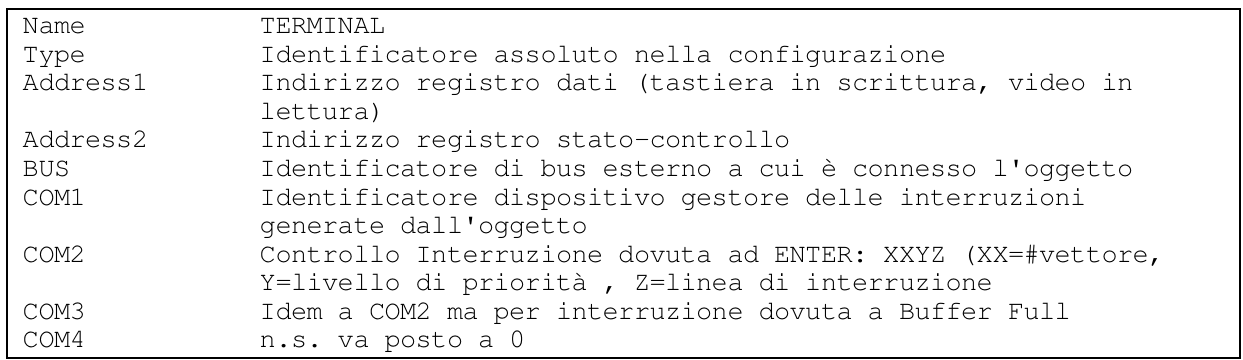
\includegraphics[width=\textwidth]{img/termianl.png}
    \caption{Configurazione di Terminal}
    \label{img:cfg_terminal}
\end{figure}

\begin{figure}[h!]
    \centering
    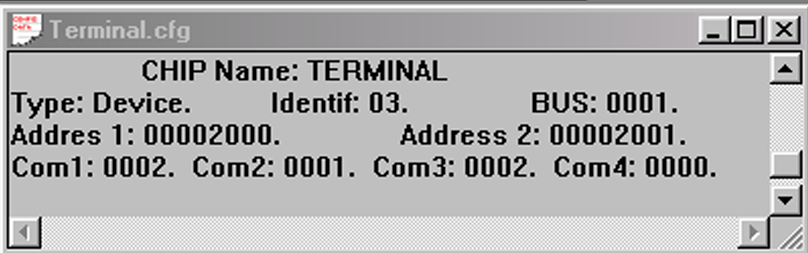
\includegraphics[width=.8\textwidth]{img/terminal_type_cfg.png}
    \caption{Configurazione tipica di Terminal}
    \label{img:cfg_terminal1}
\end{figure}

La tastiera accetta caratteri solo se abilitata e l'input va a video solo se la funzione di \textit{echo} è attiva. Queste funzionalità sono disabilitate di default, quindi quando si accende la macchina è opportuno che il processore esegua una configurazione accedendo in scrittura al registro CTRL. Si tratta di un registro di un solo byte, così configurabile:

\begin{table}[h!]
    \centering
    \begin{tabular}{|m{0.5cm}|m{1cm}|c|}
        \hline
        \multirow{6}{*}{\rotatebox{90}{Controllo}} & \textbf{bit 0} & Se alto, abilita l'interruzione \textit{buffer full} \\
        \cline{2-3}
        & \textbf{bit 1} & Se alto, abilita l'interruzione sul tasto \textit{Enter} \\
        \cline{2-3}
        & \textbf{bit 2} & Cancella il video \\
        \cline{2-3}
        & \textbf{bit 3} & Pulisce il buffer da tastiera \\
        \cline{2-3}
        & \textbf{bit 4} & Abilita la tastiera \\
        \cline{2-3}
        & \textbf{bit 5} & Abilita l'echo \\
        \hline
        \multirow{2}{*}{\rotatebox{90}{Stato}} & \textbf{bit 6} & Stato di buffer Full \\
        \cline{2-3}
        & \textbf{bit 7} & Stato di Enter inviato \\
        \hline
    \end{tabular}
\end{table}

Terminal possiede due indirizzi di accesso: il primo, associato al buffer di tastiera e video, mentre il secondo al registro CTRL (controllo/stato). Un'operazione di accesso in scrittura sul primo  indirizzo comporta la stampa a video del carattere scritto; i caratteri validi sono quelli  con codice ASCII compreso tra 32 e 126 (estremi inclusi) ed il carattere con codice 13 che provoca il ritorno a capo. Quando una riga è piena, il successivo carattere viene scritto nella riga 
seguente; se tutte le dieci righe sono piene il testo scorre di una riga verso l'alto. Ponendo ad 1 il bit 2 di CNTRL, 
si pulisce lo schermo e si riporta il cursore in alto a sinistra. 

Un'operazione di accesso in lettura sul primo indirizzo consente di prelevare un carattere dal buffer di tastiera. 
Partendo dallo stato di buffer di tastiera vuoto e con tastiera ed eco abilitati, si digiti una frase qualsiasi. Per ogni carattere premuto, il corrispondente carattere va nel buffer di TERMINAL ed appare nella finestra; inoltre il 
numero di caratteri nel buffer si incrementa di un'unità. Se vengono battuti più di 256 caratteri la tastiera viene 
disabilitata, il bit 6 di CNTRL va ad 1 e, se il bit 0 è alto, viene inviata un'interruzione per segnalare al processore la condizione di "Buffer full". Quando si è completata la frase (con meno di 256 caratteri) va premuto il tasto di ENTER; ciò porta TERMINAL a disabilitare la tastiera, ad alzare il  bit 7 di CNTRL ed ad inviare al processore un' interruzione se il bit 1 di CNTRL è alto; ogni qualvolta il processore legge un carattere dal buffer, il numero di caratteri letti, inizialmente nullo, si incrementa di uno; tale numero rappresenta un puntatore al primo carattere non letto e, il fatto che si incrementi man mano, fa si che il processore legga, nel  corretto ordine, tutti i caratteri nel buffer. L'ultimo carattere è sempre l'ENTER; per riattivare la tastiera e pulire il buffer occorre portare al valore 1 i bit 3 e 4 di CNTRL. 
Ponendo a 0 il bit 5 di CNTRL si disabilita l'eco; ciò è utile quando si vuole nascondere l'input di tastiera come 
nel caso in cui venga digitata una password. 





